\chapter{Introduction}

\paragraph{Assurance is the key to unlocking autonomy} Over the last decade, there has been an explosion in the capabilities of autonomous systems and artificial intelligence. While autonomous systems are becoming more tightly integrated into our daily lives, there is still a gap between their technological capabilities and their actual impact. The use of autonomous systems today provide just a glimpse of the potential that the broader deployment of autonomy in society has to drive economic growth and productivity. 



However, the growing scale of impact of autonomous systems in society means that the consequences of the failure of these systems are correspondingly large. Guaranteeing safety and reliability for increasingly complex systems only grows more challenging whilst simultaneously becoming more crucial for their adoption in society. Studies have shown that user concerns over safety, and more broadly, \emph{lack of trust that the system will meet expectations} remains the most significant barrier to deployment for autonomous systems~\cite{KAUR201887,BEZAI202165,MOLNAR2018319}.  


Broad adoption of autonomous systems can provide solutions for emerging societal issues such as congestion~\cite{LIORIS2017292,8734238}, smart urban planning~\cite{GULSRUD201885,NITOSLAWSKI2019101770}, climate change~\cite{KOLOKOTSA2017101,goddard2021global}, and many others~\cite{DUONG2020355}. It is thus necessary to \emph{provably guarantee} to regulators and build trust with consumers that the risk of failure is minimal. Hence, there is a strong need to develop systematic approaches to verify that autonomous systems will comply with all regulations, keep humans safe, and achieve their missions. \emph{Assured autonomy}, where an autonomous system is formally and provably guaranteed to meet precisely stated objectives, is the key to unlocking the full impact that autonomy can bring to our society. 

Assured autonomy has attracted immense interest from government, industry, and academia. It is being widely studied in various contexts as they relate to autonomy including perception, control, learning, motion-planning and decision-making. The focus of the work in this dissertation is on \emph{assured decision-making}. While this concept will be more formally explained in the following sections, I informally state here that assured decision-making is the problem of guaranteeing that the decisions made by an autonomous system will lead to the specified outcome. In the following sections I will lay out formally lay out how I model the decision-making process of an autonomous agent, and the methods by which we assure the decisions lead to desired outcomes. 


\subsection{What is decision-making?}

The decision-making process for an autonomous agent is shown in Figure~\ref{fig:decisionloop}. The agent must use its sensors to \emph{observe} the state of the environment. It then processes the information and makes a \emph{decision} to perform an action which its control surfaces must enact.
\begin{figure}
	\centering
	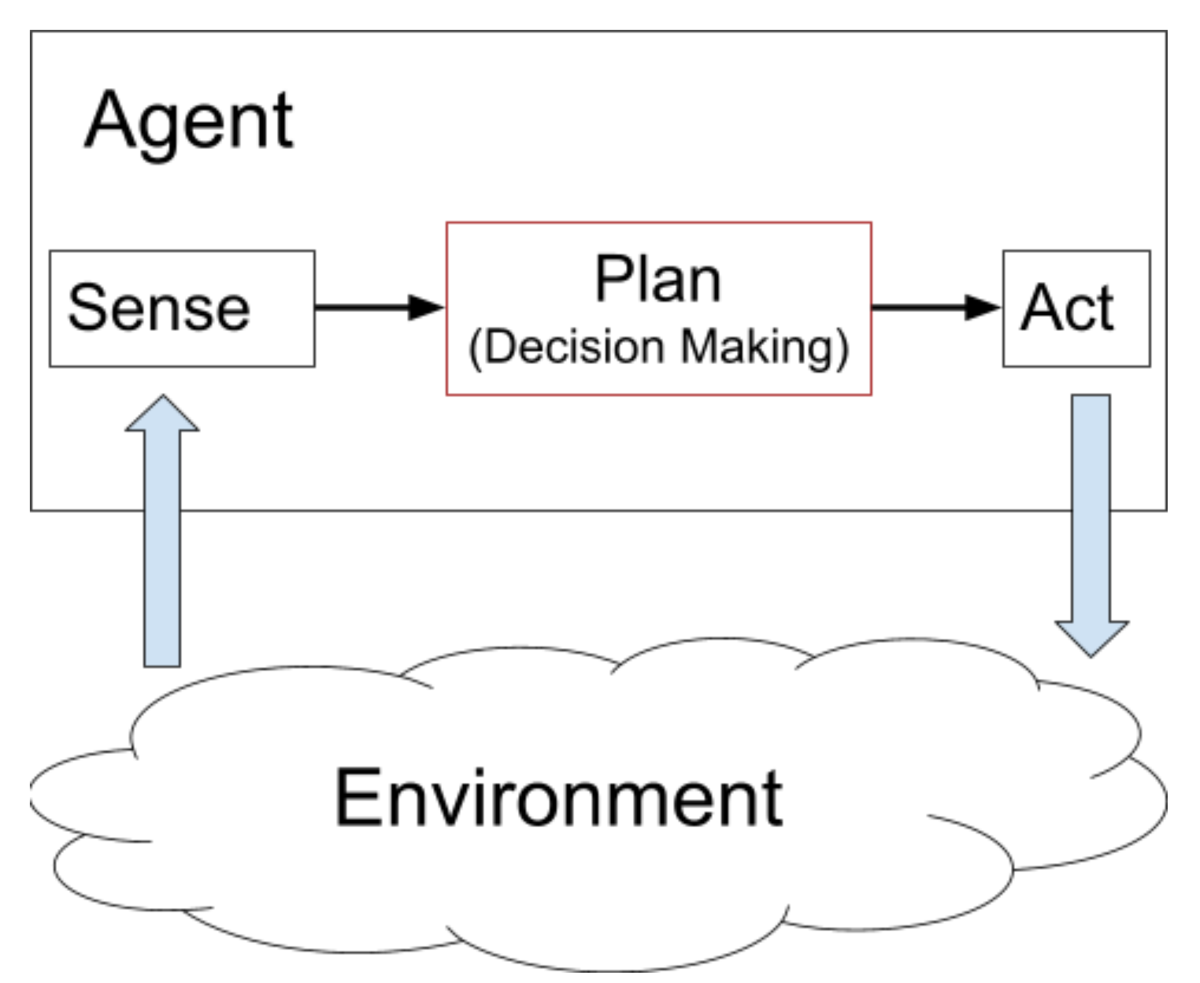
\includegraphics[width=0.5\linewidth]{Introduction/Figs/decisionloop}
	\caption{Simplified process illustration for an autonomous system interacting with the environment.}\label{fig:decisionloop}
\end{figure}


The goal of the decision-making module is to use the information from the sensors to \emph{decide} what action the autonomous agent must make that its control actuators can feasibly implement in order to achieve some higher-level objective. 

In this dissertation, I address the following research questions in the context of decision-making

\begin{itemize}
	\item \emph{How can we specify complex tasks to autonomous agents in a formal but intuitive way with quantitative performance guarantees?}
	\item \emph{How can we provide provable guarantees on the abilities of autonomous agents to carry out these complex tasks?}
	\item \emph{How can users qualitatively tune the behaviour of the agents carrying out these tasks?}
\end{itemize}


\subsubsection{Decision-making in the autonomy stack}


Most complex autonomous systems are made up of several modules designed by different teams. For example, perception, controls, path-planning, decision-making can all be different parts of the stack. It is thus important that any decision-making module fit in the architecture of an autonomy stack without requiring the full implementation details of the rest of the system. For example, the module must not rely on the precise sensors or algorithms used in the perception stack. In my work, I show that the assurance processes are designed \emph{agnostic} to the specifics of the other modules. The goal of my work is to \emph{assure} that the decison-making method (shown in the red-box in Figure~\ref{fig:decisionloop}) is guaranteed to lead to the specified outcome.  

The decision-making method must of course take into account the capabilities of the sensors and actuators in order to ensure the decisions it makes are actually feasible to implement. For example, in Chapter~\ref{sec:SurveiilanceChapter}, I discuss my work on autonomous surveillance where the agent cannot always sense the location of the adversaries. The work I will present focuses on the case where there is some characterization of the sensing and control capabilities (or lack thereof) and how to guarantee the decisions made with that understanding will lead to the specified objectives. I note for emphasis, that the algorithms provided in this paper, do not depend on the specific characterizations of the capabilties - the guarantees change based on what the system is able to feasibly implement. 

\subsubsection{Specifying objectives}

Formally specifying precise, verifiable outcomes for the behaviours of autonomous systems is a challenging task. The challenge is further exacerbated by the fact that it will be necessary for non-expert users to interact with and direct increasingly autonomous systems. Non-expert users will need to specify complex tasks to autonomous agents in a precise, but intuitive way, while additionally being able to direct qualitative behavior. 

To illustrate this concept, take for example, an autonomous home vacuum cleaner. The owner may want to issue instructions to vacuum the entire home and additionally specify the order in which the rooms are cleaned. In this example, the owner can state a precise outcome - \emph{vacuum the entire home}, and then tune qualitative behavior of the agent in achieving the outcome - \emph{clean the kitchen first, then the living room, then the bedroom}. 

Furthermore, the ability for non-expert users to specify and tune high-level behavior is crucial from the context of regulation and certificiation. For more complex autonomous systems such as autonomous vehicles or aircraft to be deployed, regulations (written in natural language) must be shown to be adhered to. For example, a regulator may require verification that \emph{no more than X drones are allowed to occupy Y region of airspace}. Again, this is a high-level requirement that the autonomous system must verifiably follow. 

There is not one-size-fits-all approach to formal objective specification. Different applications will have different approaches that are best suited for them. The work in this dissertation relies on the specification provided in temporal logic. I argue that, while this is still a mathematical representation, it is significantly more intuitive to handle compared to manually engineering reward functions (which is standard practice in the AI domain). The long-term goal for assurance is to be able to assure objectives provided in natural language, but that is outside the scope of this dissertation. 

%Of course, this statement leads to questions like: \emph{what does it mean when an autonomous sysem makes a decision?} and \emph{how does one "specify" an outcome?}. These questions have different answers based on the specifics of the context in which they are being asked. I will 




%In order for autonomous systems to become more tightly integrated in society, they will need to be able to handle tasks with increasing levels of complexity. Furthermore, it will be necessary for these systems to interact with non-expert users. As human reliance on autonomy grows, it is also necessary to have \emph{guarantees} on the abilities of these systems to achieve their missions. In this context, we are interested in the following questions:
%\begin{itemize}
%	\item \emph{How can we specify complex tasks to autonomous agents in a formal but intuitive way with quantitative performance guarantees?}
%	\item \emph{How can we provide provable guarantees on the abilities of autonomous agents to carry out these complex tasks?}
%	\item \emph{How can users qualitatively tune the behaviour of the agents carrying out these tasks?}
%\end{itemize}





\subsection{Assurance through synthesis}

Testing and simulation are logical methods in determining the safety of an autonomous systems. For example, makers of self-driving cars rely on test-driving their cars in real traffic and gathering data. However, studies have shown that the amount of real-world testing needed to truly be confident in a system's safety is not practical and have called for more \emph{innovative methods of demonstrating safety and reliability}~\cite{KALRA2016182}. 

In this dissertation, I draw from the field of \emph{formal methods} to provide formal guarantees. Techniques from formal methods have been widely used in software verification with great success. These techniques are being increasingly applied to autonomous robotics systems. However, there are several challenges that limit the use of formal methods in robotics and autonomy which are detailed in~\cite{10.1145/3342355}. I refer the reader to ~\cite{10.1145/3342355} for full details, but in short, issues such as objective specification, environment modelling, and multi-agent systems are all open challenges in the use of formal methods in assuring autonomous systems. Often, these issues are domain-specific and there is no generalized solution. In my work, while there are some domain-specific modeling needed (i.e., in Part III for urban air mobility), I provide solutions for general theoretical problems such as guarantees under partial-information and safety in multi-agent settings and demonstrate the results in specific applications. 

Broadly, we can provide assurances either by \emph{verifying} a system adheres to specifications or by \emph{synthesizing} the system from the specification that guarantees correctness. Both methods are widely applied in different areas, but in this dissertation I focus on \emph{synthesis} based approaches.

This is because one drawback of verification methods is that it cannot construct a new system if the existing system does not meet the given specifications. Synthesis, on the other hand, is \emph{correct-by-construction}, i.e., it constructs a system directly from the given specifiacitons that is guaranteed to be correct. However, synthesis techniqes suffer from scalability concerns that limit its ability to be employed in more realistic settings, especially those involving partial-information or multiple agents. Often, abstraction techniques and decentralized architectures are necessary for synthesis techniques to be computationally feasible. In this dissertation, I present my work in employing scalable synthesis approaches to generating complex systems with guarantees of correctness with respect to specifications. In particular, I will show how these techniques can be instrumental in providing a systematic and rigorous pathway to certification and deployment of increasingly autonomous systems in safety-critical contexts.  


\subsection{Assured autonomy for urban air mobility} One application area in which autonomy is poised to make a fundamental impact is urban air mobility (UAM). Mass transportation of both passengers and cargo using increasingly autonomous air vehicles in metropolitan areas is an imminent possibility. For such an expansive vision to be realized, there are a significant number of technical challenges to be addressed.  First and foremost is the issue of safety. With projections indicating high-volume use of autonomous aircraft in urban air spaces, it is clear that advances in decision-making for autonomous systems with \emph{assured performance} will play a key role in the advancement and acceptance of UAM. Furthermore, any such technical solution must be able to handle the envisioned massive scale of operations as well as communication and sensing restrictions. Second, in any large-scale operations involving autonomy, it will be necessary for non-expert users to interact with and direct increasingly autonomous systems. However, specifying a complex mission is no trivial task and can often require extensive tuning and expertise. 


\subsection{Structure}

The dissertation is divided into 3 parts. In Part I, I will present my work on \emph{design-time synthesis}. Specifically, I focus on the application area of autonomous surveillance against adversarial moving targets. I also present our work on incorporating information gained at runtime into design-time synthesis to improve performance while still providing guarantees of correctness. 

In Part II, I discuss my work on \emph{multi-agent runtime assurance}. I will first present our work on \emph{quantitative shielding}, i.e., minimizing an interference cost function while still guaranteeing safety at runtime. However, this work suffers from scalability concerns which I address in Chapter 5 by providing a decentralized algorithms with guarantees of fairness and correctness.

Finally, Part III combines the contributions from Parts I and II into assurance methods for traffic management in urban air mobility. I show how we can use both design-time synthesis as well as multi-agent runtime assurance in order to design a synthesis architecture that can scalably guarantee safe operations for urban air mobility. 


% Metropolitan areas (other areas more scope)
%%%% Combine is too weak 
%% Learning theory 

%\paragraph{Technical contributions} In my research, I have employed an interdisciplinary approach to address the technical challenges of assuring autonomy for large-scale complex systems. Specifically, I formulate techniques that draw from formal methods, learning theory, and controls. The field of formal methods is a powerful tool for providing guarantees on performance and safety. However, it suffers from a lack of scalability, restricting its use in partial-information or multi-agent settings. I have designed algorithms that leverage the guarantees of formal methods with the efficiency of techniques in controls and learning to perform complex missions with provable guarantees in large environments. For example, I have designed algorithms for multi-agent surveillance tasks, large-scale traffic management for UAM, safe learning for multiple agents, and others. Providing high-level mission guarantees in such settings was previously beyond the reach of standard approaches in formal methods due to state-space explosion and lack of automated techniques. In my research I have shown not only theoretical guarantees of safety and performance, but also real-world applicability with high-fidelity simulations in collaboration with industry partners such as NASA and Skygrid, as well as experiments on hardware with Sandia National Labs.
